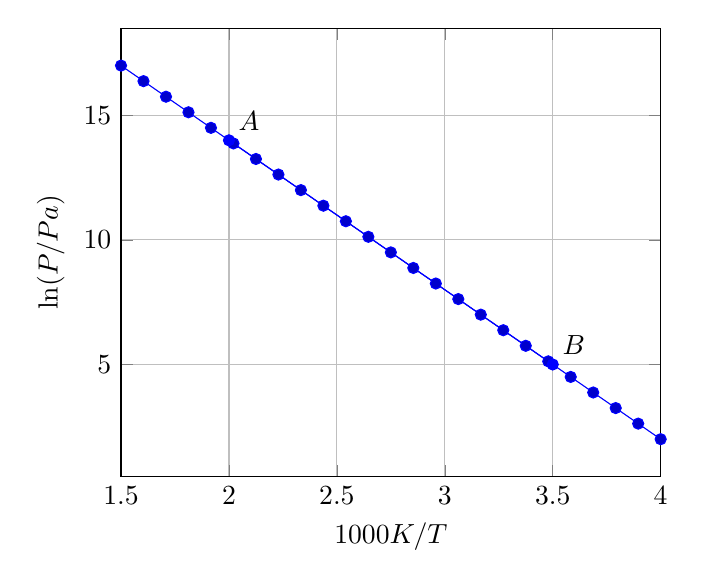
\begin{tikzpicture}
    \begin{axis}
        [
            grid = major,
            xlabel = {$\qty{1000}{K}/T$},
            ylabel = {$\ln (P/\unit{Pa})$},
            xmin = 1.5, xmax = 4,
            domain = 1.5:4,
        ]

    \addplot
        { -6*x + 26 };

    \addplot [mark=*, color=blue] coordinates
        { 
            (2,14)
            (3.5,5) 
        };

    \node [anchor = south west] at (axis cs:2,14) 
        {$A$};

    \node [anchor = south west] at (axis cs:3.5,5) 
        {$B$};

    \end{axis}
\end{tikzpicture}